\documentclass{article}
\usepackage[utf8]{inputenc}
\usepackage{times}
\usepackage[titletoc]{appendix}
\usepackage{graphicx}
\usepackage{lineno}
\usepackage{multirow}
\usepackage[english]{babel}
\usepackage{typearea} 
\usepackage{amssymb}
\usepackage{amsfonts}
\usepackage{amsmath}
\usepackage{enumerate}
\usepackage{mathtools}
\usepackage{graphicx}
\usepackage{wrapfig}
\usepackage{lscape}
\usepackage{rotating}
\usepackage[colorinlistoftodos]{todonotes}
\newcommand{\Fig}[1]{Figure~\ref{fig:#1}}

\renewcommand{\baselinestretch}{1.5}
\newcommand{\bbar}[1]{\overline{#1}}

\newcommand\scalemath[2]{\scalebox{#1}{\mbox{\ensuremath{\displaystyle #2}}}}
\renewcommand{\familydefault}{\sfdefault}

\usepackage[font={small},labelfont={bf},justification=justified,margin=0.5cm]{caption}

\renewcommand{\thesection}{}
\renewcommand{\thesubsection}{\arabic{section}.\arabic{subsection}}

\usepackage{color}
	 \definecolor{darkred}{rgb}{0.9,0,0}
%	 \definecolor{darkgreen}{rgb}{0,0.5,0}
	 \definecolor{darkblue}{rgb}{0,0,0.75}
%	 \definecolor{magenta}{rgb}{0,0,0.75}
\newcommand{\hhone}{(H,H,1)}
\newcommand{\hhtwo}{(H,H,2)}
\newcommand{\hsone}{(H,S,1)}
\newcommand{\hstwo}{(H,S,2)}
\newcommand{\shone}{(S,H,1)}
\newcommand{\shtwo}{(S,H,2)}
\newcommand{\ssone}{(S,S,1)}
\newcommand{\sstwo}{(S,S,2)}

\newcommand{\hhstar}{(H,H,$\star$)}


\usepackage{hyperref}
\definecolor{darkgreen}{rgb}{0.1,0.6,0.3}
\definecolor{darkred}{rgb}{0.6,0.3,0.1}
\hypersetup{
    colorlinks=true,       % false: boxed links; true: colored links
    linkcolor=blue,          % color of internal links (change box color with linkbordercolor)
    citecolor=darkgreen,        % color of links to bibliography
    filecolor=magenta,      % color of file links
    urlcolor= black           % color of external links
}


% remove this before we submit...
\definecolor{greenie}{rgb}{0.1,0.62,0.0}
\definecolor{orange}{rgb}{0.9,0.3,0.0}
\definecolor{deepblue}{rgb}{0.0,0.0,0.7}
\newcommand{\marcus}[1]{{\color{orange}{#1}}}
\newcommand{\chaitanya}[1]{{\color{greenie}{#1}}}
\newcommand{\cha}[1]{\textcolor{darkgreen}{(#1)}}
\newcommand{\joe}[1]{{\color{deepblue}{#1}}}

\title{\vspace*{-22mm}\bf Title}
%\author{Chaitanya S. Gokhale$^{1}$, Joseph Bulbulia$^{2,3}$, Marcus Frean$^{4}$\\
%\normalsize $^1$Research Group for Theoretical Models of Eco-evolutionary Dynamics\\
%\normalsize Department of Evolutionary Theory, \\
%\normalsize Max-Planck Institute for Evolutionary Biology, 24306 Pl\"{o}n, Germany, \\
%\normalsize $^2$School of Humanities, Faculty of Arts, University of Auckland, New Zealand \\
%\normalsize $^3$Max Planck Institute for the Science of Human History, Jena, Germany \\
%\normalsize $^4$School of Engineering and Computer Science, \\
%\normalsize Victoria University of Wellington, New Zealand
%}


\date{}

\begin{document}

\linenumbers
\maketitle

\begin{abstract}
% Suggest we set this up differently:
Abstract stuff
\end{abstract}


\noindent
Keywords: social evolution, culture, narratives, stag-hunt


%\tableofcontents

\section{Introduction}
gwbniwbwnijb
\cite{skyrms:book:2003}

%\textbf{Collective cooperation and resource dynamics}.
%

\section{The dynamics stag hunt}

Replicator dynamics is the core idea of evolutionary dynamics. Replicator dynamics determines how the frequency of different strategies in a population changes over time.
We can analyze the equation used to determine replicator dynamics mathematically.
Let's take the frequency of $a$ and $b$ strategies are $x_a$ and $x_b$ and the fitness of each strategy is $f_a$ and $f_b$. It is a two-player game so we can say, $ x_a+x_b=1 $. We can write two differential equations using the above information
\[
{dx_a}/{dt} = x_a(f_a - \bar{f})    (1)
\] 
\[{dx_b}/{dt}= y(f_b - \bar{f})   (2)
\].
Now to keep the average fitness of the population constant, we can write an equation,
\[\bar{f}= (x_af_a+x_bf_b)   (3) \],
also, we can write the previously mentioned equation as $x_b=1-x_a$.
Now, we can substitute this $x_b$ value into the $3$ numbered equation, after substituting, we get the undermentioned equation.
\[\bar{f}={x_af_a+ (1-x_a)f_b} (4) \]
Now let's substitute the $(4)$ numbered equation into the $(1)$ equation
\[ dx_a/dt=x_a[f_a-(x_af_a+(1-x_a)f_b)]
          =x_a[f_a-x_af_a-f_b+x_af_b]
          =x_a[(1-x_a)f_a-(1-x_a)f_b]
          =x_a(1-x_a)(f_a-f_b) \] .
This is for a two-player population. If we have $n$ population, we can denote the equation of replicator dynamics as,
\[dx_i/dt=x_i[f_i(x)-\bar{f}]\]
where $i=1,2,3.....(n-1)$

To proceed with the replicator dynamics, we must understand simplex as the next step.
Simplex is a tool in evolutionary dynamics that helps us understand and visualize how a system evolved through an evolutionary process. We can denote this for $(n-1)$ strategies. But for simplicity, we took a two-player ($n=2$) homogenous process in which for $a$, $x_a=1$ and $x_b=0$, or the same goes for $b$, where, $x_a=0$ and $x_b=1$.
It will represent a line between points $a$ and $b$, with the midpoint being $x_a=x_b=0.5$. 
For another example, if we homogeneously use $ n=3$, it will represent an equatorial triangle, and the midpoint of the simplex will be $x_a=x_b=x_c=1/3$.
In population genetics, this simplex is known as the de Finetti diagram.
Let's get back to the replicator dynamics now,
\[dx_a/dt=x_a(1-x_a)(f_a-f_b)\],
What does this equation tell us? 
We can understand that the rate of change of the frequency of a certain type with time depends on the fitness, average fitness of the population, and frequency. From this understanding, we can state that if $f_i(x)-\bar{f}>0$ then the frequency of this type will increase over time, and if $f_i(x)-\bar{f}<0$, the frequency of the type will decrease over time.
If we make the change of strategy $a$ over time constant, which means $dx_a/dt=0$ then we can write the replicator dynamics equation as,
\[x_a(1-x_a)(f_a-f_b)=0\]
Now, if we try to find the certain under which $dx_a/dt$ will be $0$.
We will have three certain conditions,
\[x=0,x=1\] and \[f_a=f_b\]
$x=0$ and $x=1$ will be the two end points of a single line simplex and the joining point for the frequency graph and the dynamics of this frequency depends on the values of $f_a$ and $f_b$. If $f_a>f_b$ then the curve will be over the $0$ if $f_a<f_b$ then the curve will be under $0$, and for the condition $f_a=f_b$, it will make a straight line between the $0$ and $1$.For a visual representation of this graph, we can plot this equation for different values of $f_a$ and $f_b$ using Python.
\begin{figure}[h]
        \centering
        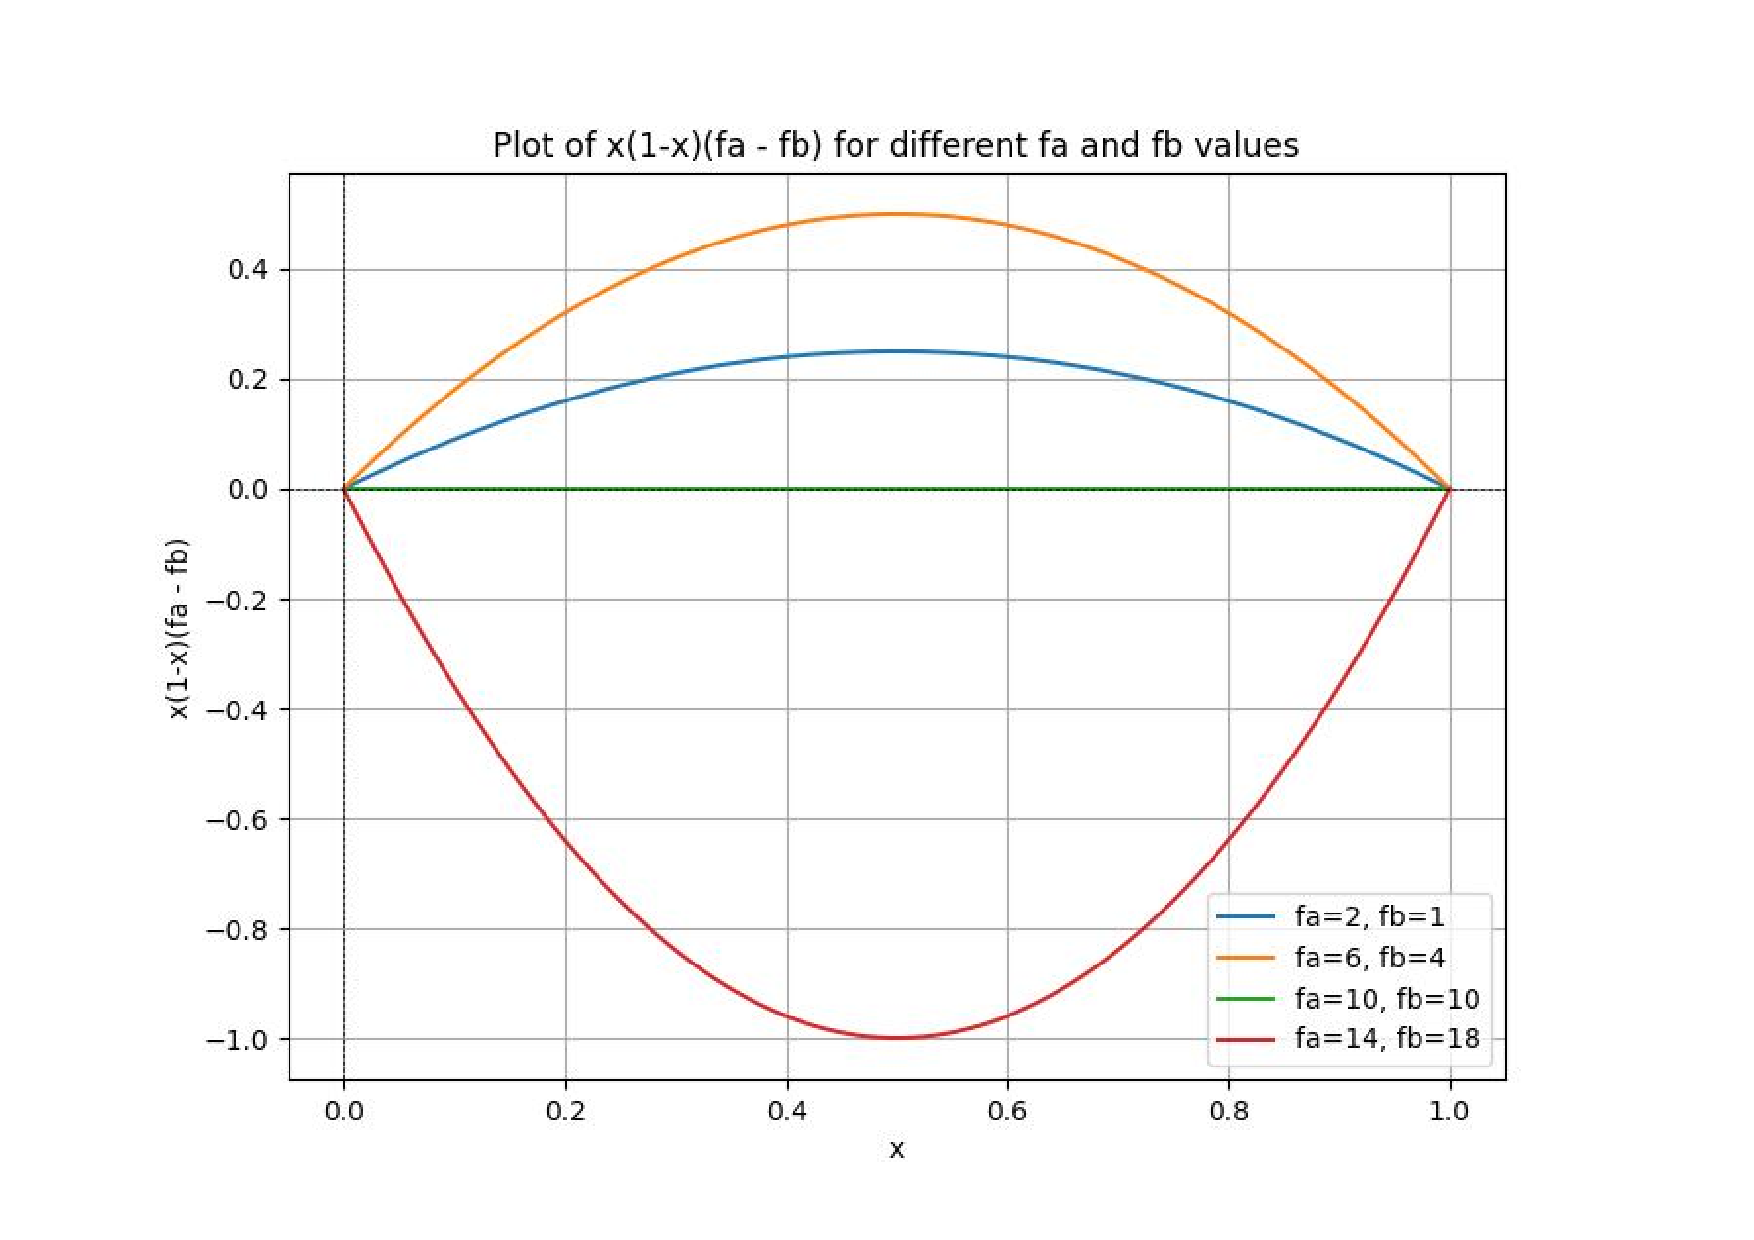
\includegraphics[width=0.5\linewidth]{Figure_1.png}
        \label{fig:Visualization of $x_a(1-x_a)(f_a-f_b)=0$}
    \end{figure}
We can get different conditions from this equation and graph. 
(1) Dominance: Where any of the two strategies will be dominant over another, means, for example if $f_a>f_b$ then strategy $a$ will be dominant over strategy $b$. It will be possible if the $a_1>b_1$ and $a_0>b_0$ where $a_1,a_0,b_1,b_0$ are the payoffs of a payoff matrix of a two-player game.
(2) Co-existence: It happens when one of the two strategies is rare and has an advantage for that. For example, if strategy $a$ is rare, then $f_a>f_b$ if $a$ becomes abundant, it will lose its advantage, so the inequality will be  $f_a<f_b$ and there will be a saturation point while becoming abundant from rare when the equation will $f_a=f_b$. In this scenario, the player should play the rare strategy.
(3) Bi-stability: A condition where all $a$ and $b$ will be stable means a strategy will get an advantage if it is abundant. For example, if strategy $a$ is abundant then the inequality will be $f_a>f_b$ and if it becomes rare then the inequality will be $f_a<f_b$ and there will be a saturation point when $f_a=f_b$. For this condition, the player should play the strategy that its opponent is playing.
(4) Neutrality: Now we have one condition in which both strategies will have the same impact. It does not depend on the change on the strategy. The equation for this strategy will be $f_a=f_b$. We mentioned this neutrality condition as saturation point before.
\subsection{Stochastic Process and Finite Population}
In the previous subsection, we used an infinite population for the deterministic approach. Now, we will proceed with a finite population. There are mainly two reasons to use a finite population: first, it is realistic, and second, it is a natural way to introduce randomness into the replicator dynamics.
Now, we can consider the finite population of a specific game as $N$.Let's assume there are two strategies $a$ and $b$. Frequencies for $a$ and $b$ are $i$ and $(N-i)$. We can write the payoff matrix according to this specification,\cite{@PhdThesis{diss_mods_00006381,
  author = 	{Gokhale, Chaitanya},
  title = 	{Evolutionary dynamics on multi-dimensional fitness landscapes},
  year = 	{2011},
  publisher = 	{Christian-Albrechts-Universit{\"a}t zu Kiel},
  address = 	{Kiel},
  keywords = 	{evolutionary dynamics; evolutionary game theory},
  abstract = 	{Evolution is the common theme linking everything in biology from individual alleles to languages. Darwin believed that those who were mathematically inclined had a different insight and he regretted not having it. He probably would feel gratified knowing that now evolution has gained a solid mathematical foundation. The general principles of evolution can be represented by precise mathematical equations. Simplicity is invoked by making use of the minimum factors that matter.
But we cannot even imagine how many factors a single honeybee takes into account to vouch for a particular flower. How can we take this complexity into account if we aim at retrieving simple tractable explanations of biological principles? This thesis addresses this problem particularly in two scenarios: Static and dynamic fitness landscapes. A fitness landscape is a tool for visualising the the fitness of a population in a space in which each dimension is a trait affecting the fitness. The population is ever searching for fitness maxima on this landscape. This is the process of adaptation. In a static fitness landscape the fitness is fixed, determined by the trait combination. Here we present results pertaining to the time required for a population to move from one point to another on this landscape if the paths consists of broad valleys or narrow ridges. In dynamic fitness landscapes the fitness is a function of the population composition. Hence as the population moves over the landscape the landscape changes shape and the fitness maxima can be eternally moving. To analyse frequency dependence we employ evolutionary game theory. Traditional evolutionary game theory deals with two player games with two strategies. This thesis invokes higher dimensions and non-linearities by studying multiple players and strategies. Important results from the two player two strategy case are generalised to multiple players. Finally we employ this theoretical development to analyse a possible evolutionary application in genetic pest management.},
  url = 	{https://macau.uni-kiel.de/receive/diss_mods_00006381},
  file = 	{:https://macau.uni-kiel.de/servlets/MCRFileNodeServlet/dissertation_derivate_00003744/Gokhale_PhD_2011.pdf:PDF},
  language = 	{en}
}
}
\[
\begin{array}{c|cc}
    & a & b \\
    \hline
  a & (a_1) & (a_0) \\
  b & (b_1) & (b_0)
\end{array}
\]
Now we can denote the average payoff of $a$ and $b$ strategies as $\pi_a$ and $\pi_b$.
\[\pi_a=\frac{i-1}{N-1}a_1 + \frac{N-i}{N-1}a_0\]
\[\pi_b=\frac {i}{N-1}b_1 + \frac{N-i-1}{N-1}b_0\]
Now, a question can arise, why are we using $i-1$ instead of $i$? We have to understand that instead of an infinitely large population, we are using a real finite population and for that, we have to remove the particular individual who is observing or analysing this situation. So we use $i-1$.
In the previous work, we used fitness directly related to payoff. But in the actual population, we introduce a tunable parameter similar to the fitness which controls the game.
Nowak et al.\cite{@article{nowak2004emergence,
  title={Emergence of cooperation and evolutionary stability in finite populations},
  author={Nowak, Martin A and Sasaki, Akira and Taylor, Christine and Fudenberg, Drew},
  journal={Nature},
  volume={428},
  number={6983},
  pages={646--650},
  year={2004},
  publisher={Nature Publishing Group UK London}
}}introduced this tunable parameter as selection intensity. Because for some situations or equations, we can know the particular relation between the fitness and payoff but for most of the cases, we don't know the particular relation, we can just create a hypothesis.
\[f_i=1-w+w\pi_i\]
where $w$ selection intensity and $\pi_i$ is the payoff. The value of $w$ is bound by  $0$ and $1$. If the value is $0$ then $f_i=1$, we can deduce from this equation that for every value of $i$, we will face neutrality, and if the value is $1$, we will have $f_i=\pi_i$, now it suggests that the game payoff controls the fitness.
Now, we can move to the part of the evolutionary dynamics where, for the finite population, there's randomness involved in the population. So, we will go for the stochastic processes.
For these stochastic processes, we will focus on the Moran process. It consists of two events: birth and death. For the birth, one subject is chosen randomly, and it produces it's identical copy, and for the death process again, one random subject is chosen from the population and eliminated. It means by introducing randomness with the birth-death process now this theory can change the population with each time step, and for $N$ steps it will control a generation \cite{@book{19631602449,
author = {Moran,P. A. P.},
title = {The statistical processes of evolutionary theory.},
year = {1962},
pages = {vii + 200 pp.},
publisher = {Clarendon Press; Oxford University Press.},
language ={Undetermined},
item-type = {Book}
}}.
There are three mathematical equations that we can derive from this theory: (1) The number of $a$ individuals increases by 1; (2) the number of $a$ individuals decreases by 1; (3)The number of $a$ individuals remains neutral.\\
For the (1) scenario, we can write:
\[T_i^+=\frac{if_a}{if_a+(N-i)f_b}\frac{N-i}{N}\]
For the (2) scenario, we can write:
\[T_i^-=\frac{(N-i)f_a}{if_a+(N-i)f_b}\frac{i}{N}\]
For the (3) scenario, we can write:
\[1-T_i^+-T_i^-\]
Now what can we deduce from these equations?\\
From the (1) equation, we can say that $a$ numbered individuals can increase only when an $a$ individual is chosen for birth and an $b$ individual is chosen for death.\\
From the (2) equation, we can say that the number of $a$ decreases cause, an $a$ individual is chosen for death and an $b$ individual is chosen for birth.\\
From the (3) equation, we can deduce that no one is chosen for the birth or death process, so there's a neutrality.\\
Now, let us jump to the fixation probability.\\
In genetics, we often ask a question related to invasion of a gene, how can the gene invade another gene, and how it affect the another gene's population?
After understanding the transition probability and moran processes, we can now form a question based on the previous mentioned topic. In population of $j$ numbered $a$ individuals and $(N-j)$ numbered $b$ individuals, what is the probability that the whole population will become of $a$ individuals?
This is known as the fixation probability of $j$ numbered $a$ individuals.We can denote this fixation probability as $\rho(j)$.
Since, fixation is an absorbing state, so if all of the population once becomes $a$, it can not be revert. We can try to write a probability balance equation.
\[\rho(j)=T_i^+\rho_a(j+1)+(1-T_i^+-T_i^-)\rho_a(j)+T_i^-\rho_a(j-1)\]
This is a discrete stochastic process which we can derive using absorbing phenomenon of Markov chain processes.




\section{Discussion}


\textbf{Code availability}.
Appropriate  computer code describing the model is available at 
\texttt{ REDACTED for review}.% {\url{https://github.com/tecoevo/beliefs}}.

\section{Acknowledgements}
\texttt{ REDACTED for review}.% {\url{https://github.com/tecoevo/beliefs}}.


\bibliographystyle{naturemag}
\bibliography{et.bib}

\renewcommand{\theequation}{SI.\arabic{equation}}
\setcounter{equation}{0}

\renewcommand{\thefigure}{SI.\arabic{figure}}
\setcounter{figure}{0}

\section{Supplementary material}


\subsection{Analysis of the simple system}

\bibliography{et.bib}


\end{document}
